
\chapter{Reflections and interactions between shock waves}
\section{Graphical representation of shock waves}
	\minifig{ch9/1}{ch9/2}{0.1}{0.1}{0.45}{0.3}	
	We have seen the representation in $(\theta , \beta)$-plane, now we introduce a (u,v)-plane called \textbf{hodograph plane}. This represents the velocity before and after the shock $\vec{v}_1$ and $\vec{v}_2$ in the plane. $\vec{v}_2$ will make an angle $\theta$ with the horizontal and it can be calculated from the previous relations. There are two solutions for $\vec{v}_2$ on the graph, the weak  (the one represented on the graph above) and the strong one. The angle $\beta$ for the weak shock is the perpendicular to the straight line connecting $\vec{v}_1$ and $\vec{v}_2$. By representing the second case corresponding to a compression, we obtain a closed curve called \textbf{shock-polar}.
	
	\minifig{ch9/3}{ch9/4}{0.1}{0.15}{0.3}{0.25}	
	We can repeat this for other $M_1$ and obtain something like that. The pressure ratio can also be represented in function of $\theta$ as on the second plot. 
	
\section{The shock reflection}
\begin{center}
\begin{minipage}{0.33\textwidth}
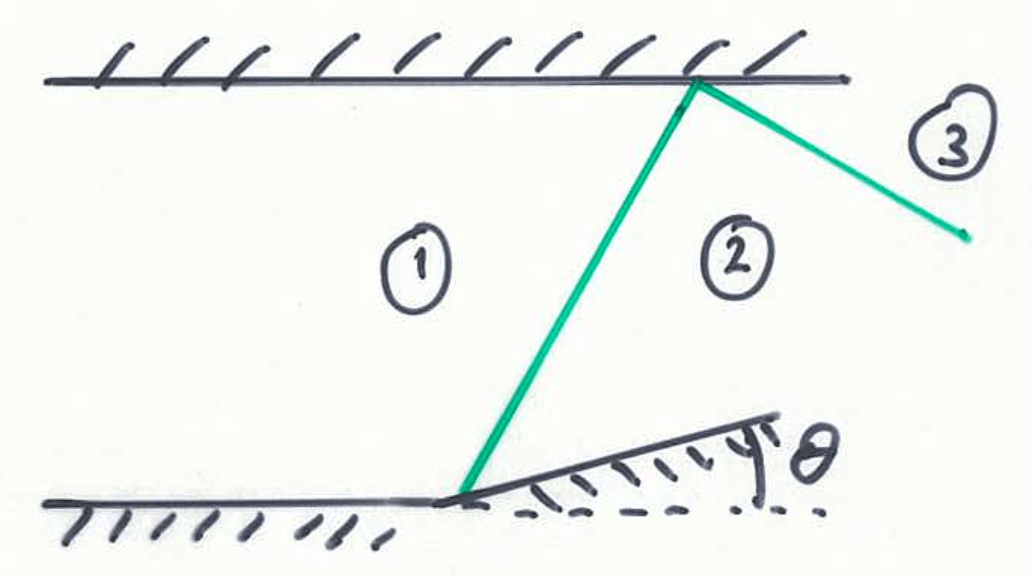
\includegraphics[scale=0.15]{ch9/5}
\captionof{figure}{}
\end{minipage}
\begin{minipage}{0.35\textwidth}
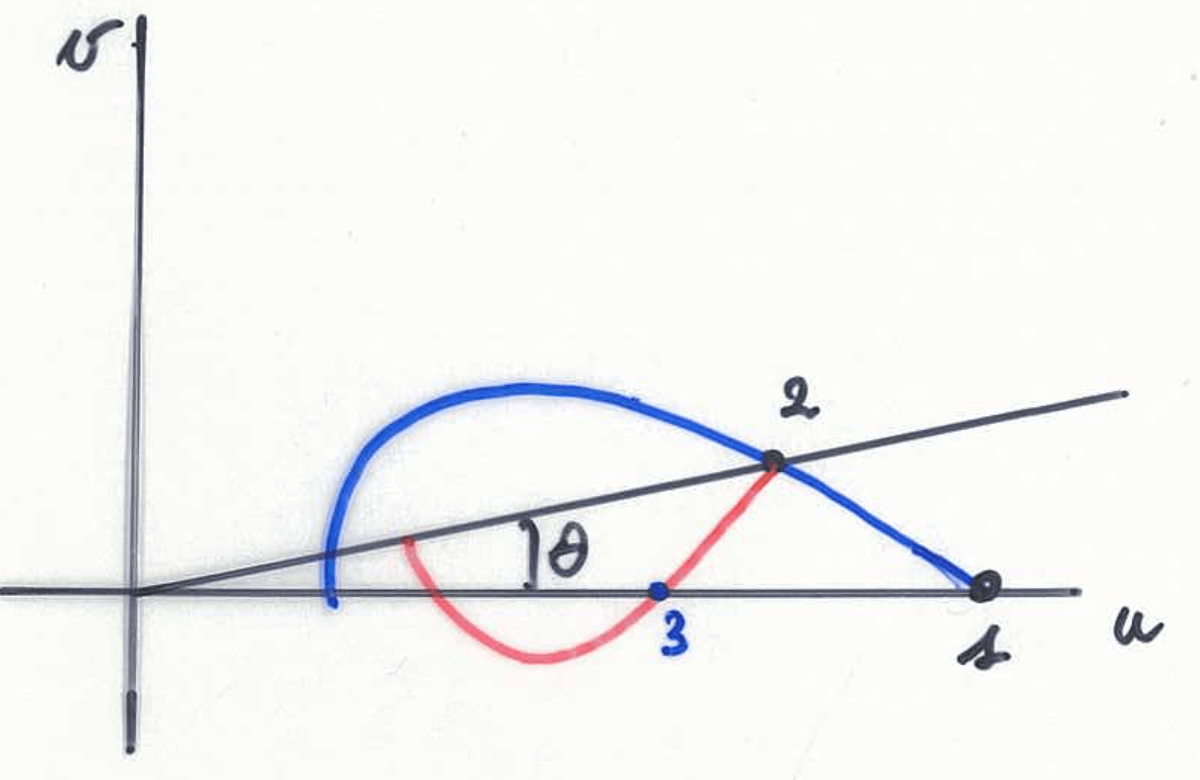
\includegraphics[scale=0.12]{ch9/6}
\captionof{figure}{}
\end{minipage}
\begin{minipage}{0.25\textwidth}
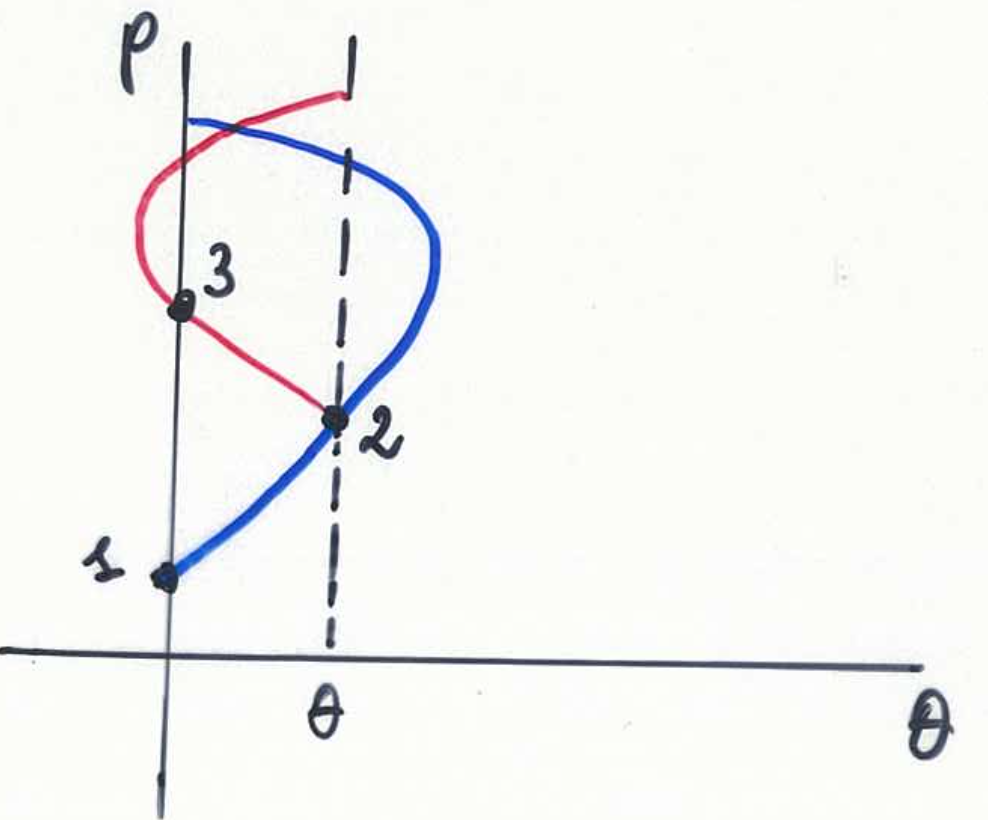
\includegraphics[scale=0.11]{ch9/7}
\captionof{figure}{}
\end{minipage}
\end{center}

The situation is represented on the first figure, the flow is first deviated by the first shock then the flow must be horizontal near the upper wall, this is possible by a second shock wave appearing at the intersection between the first shock and the upper wall (reflection shock). If this shock touches the lower wall a new shock will appear deviating the flow and so on. The velocities and the pressures can be retrieved as shown on the figures. 

\section{Crossing of shocks of different family}
\begin{center}
\begin{minipage}{0.4\textwidth}
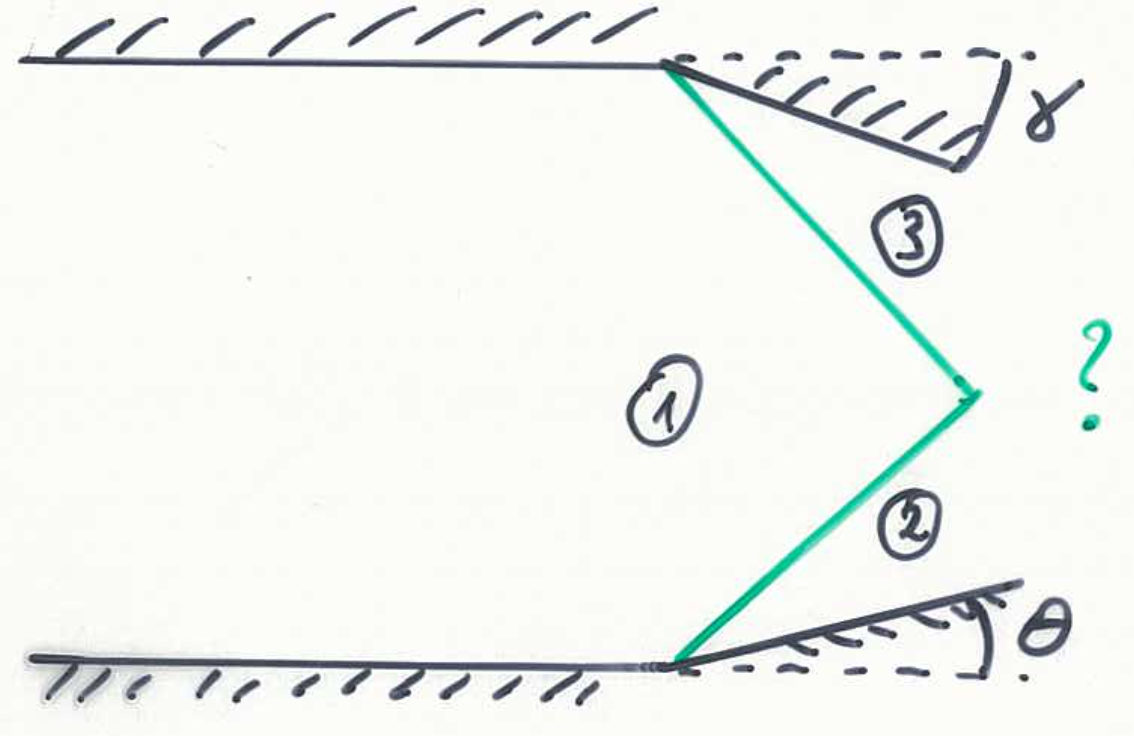
\includegraphics[scale=0.15]{ch9/8}
\captionof{figure}{}
\end{minipage}
\begin{minipage}{0.35\textwidth}
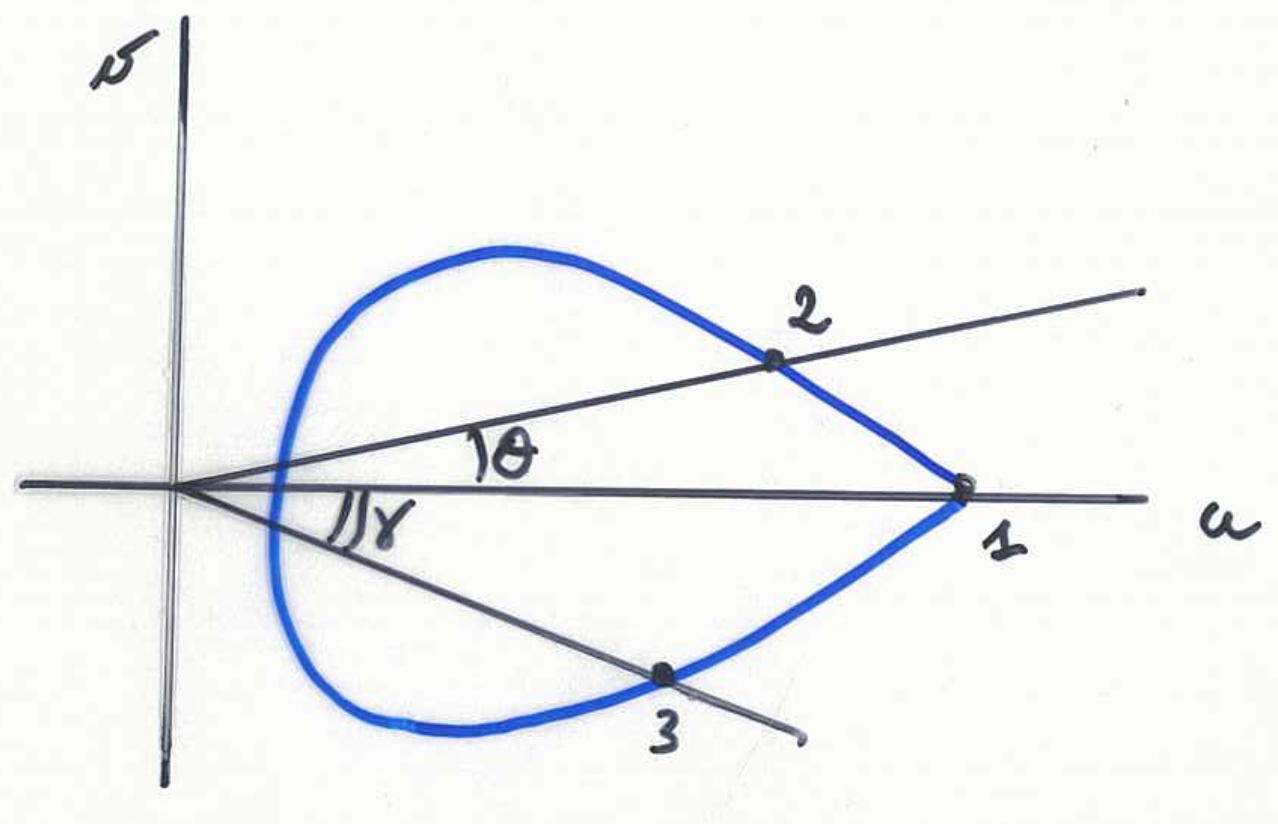
\includegraphics[scale=0.12]{ch9/9}
\captionof{figure}{}
\end{minipage}
\end{center}

Consider the situation described on the figures. We can find the solutions after each shocks individually but what happens after the cross? As the flow after each shock has a different direction, the flows cannot just join like that. The conditions to meet are:\\

\begin{itemize}
\item[•] same pressure for both flows
\item[•] the velocity direction (not the size) must be the same\\
\end{itemize}

\begin{center}
\begin{minipage}{0.33\textwidth}
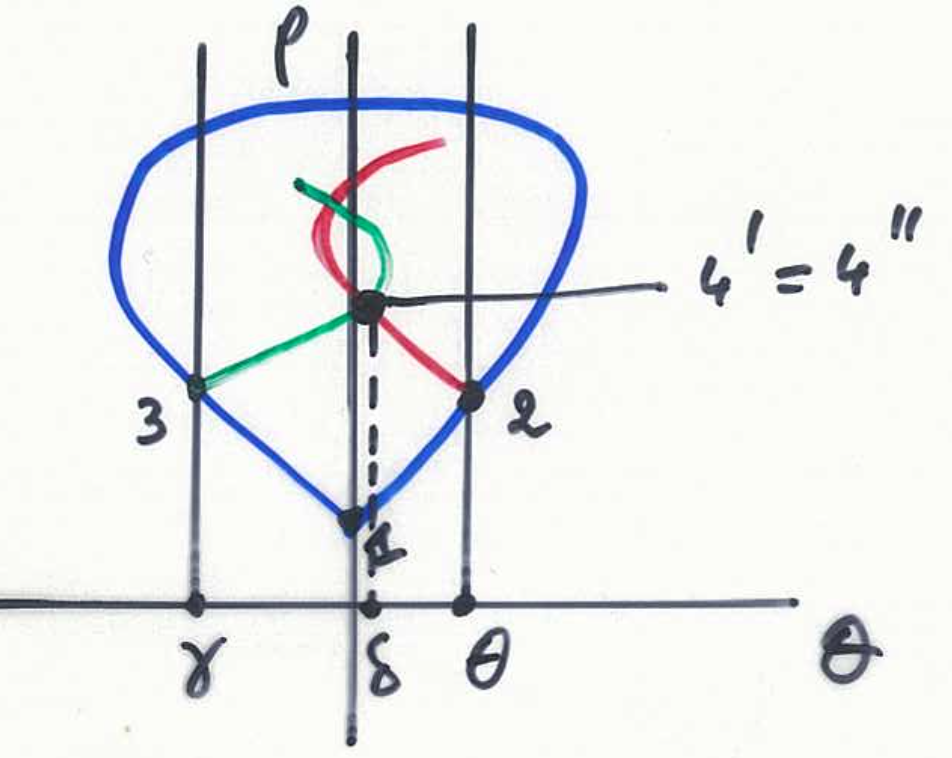
\includegraphics[scale=0.12]{ch9/10}
\captionof{figure}{}
\end{minipage}
\begin{minipage}{0.35\textwidth}
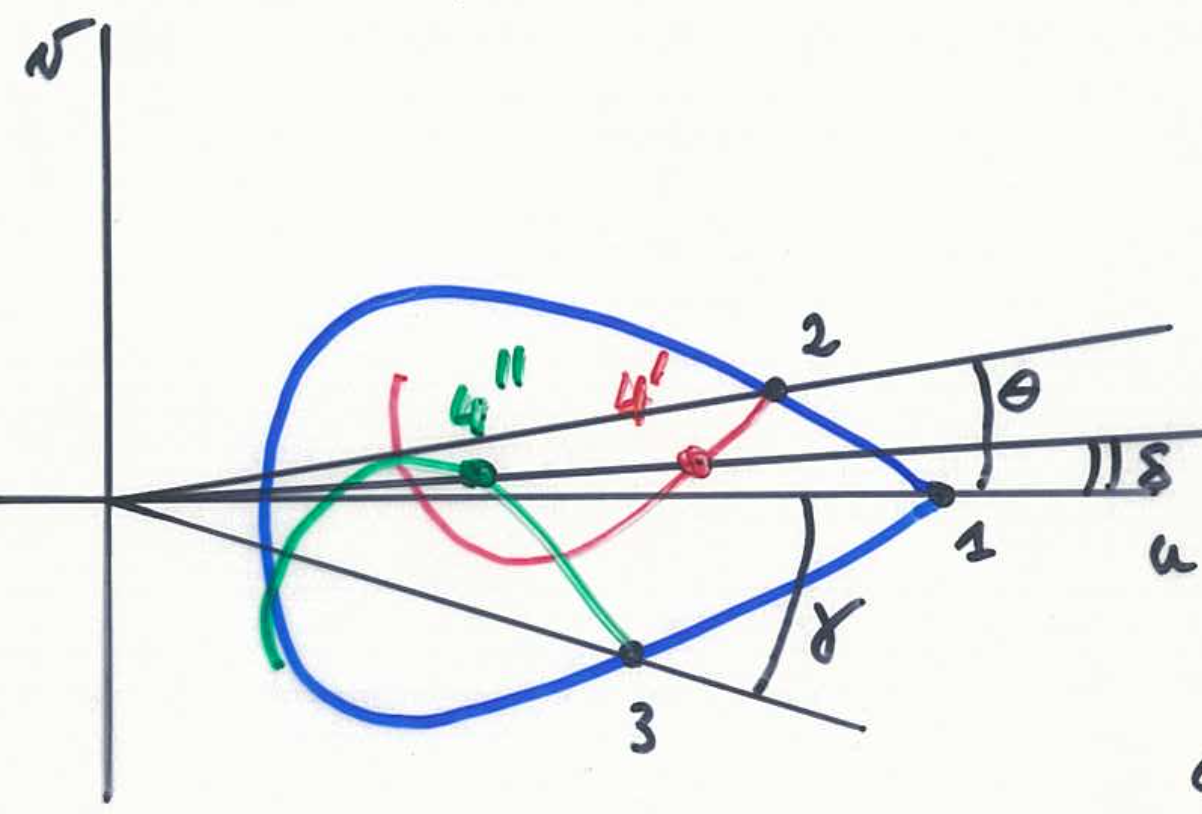
\includegraphics[scale=0.12]{ch9/11}
\captionof{figure}{}
\end{minipage}
\begin{minipage}{0.25\textwidth}
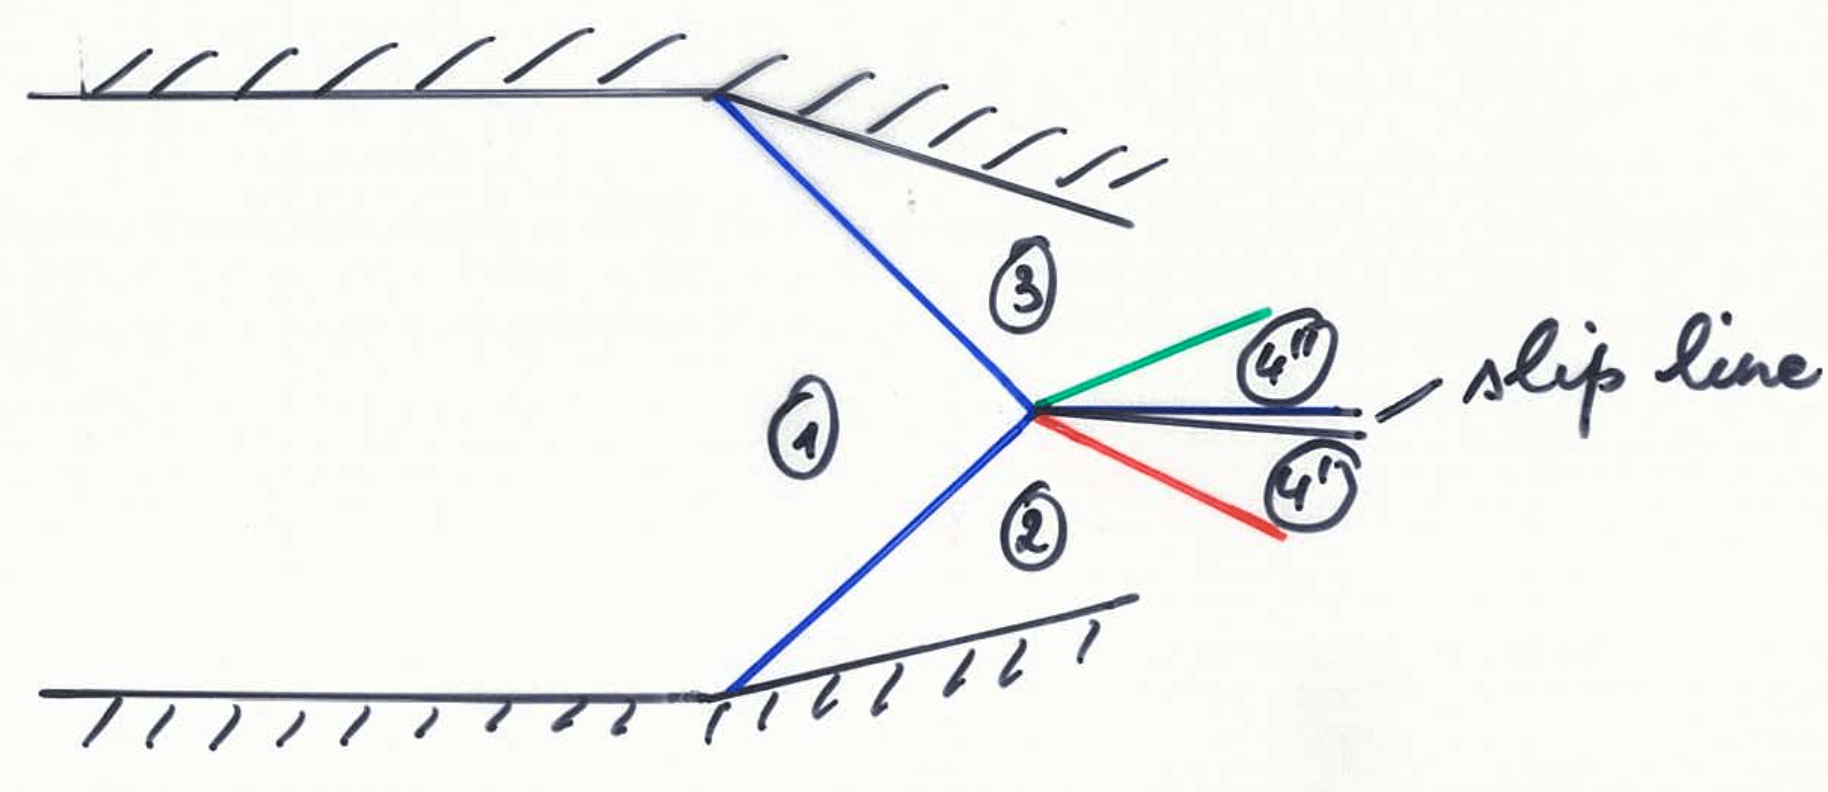
\includegraphics[scale=0.1]{ch9/12}
\captionof{figure}{}
\end{minipage}
\end{center}

The solution is that there will be reflected shocks. Thus, first of all, we have to look to the $p,\theta$ diagram and find where the curves representing situation 2 and 3 join, this determines the angle $\delta$ of the final flow. Then we can plot the straight line with angle $\delta$ on the $u,v$ diagram and find the corresponding velocities for the two shocks. We can see that the size of the velocities are different (4'' is lower), this will lead to the formation of a \textbf{slip line} of the same direction as the velocities and the starting point is the intersection of shock waves. On the figure it is represented like that because for viscous effects there will be mixing and increasing viscous layer.  

\section{Mach reflection}
\begin{center}
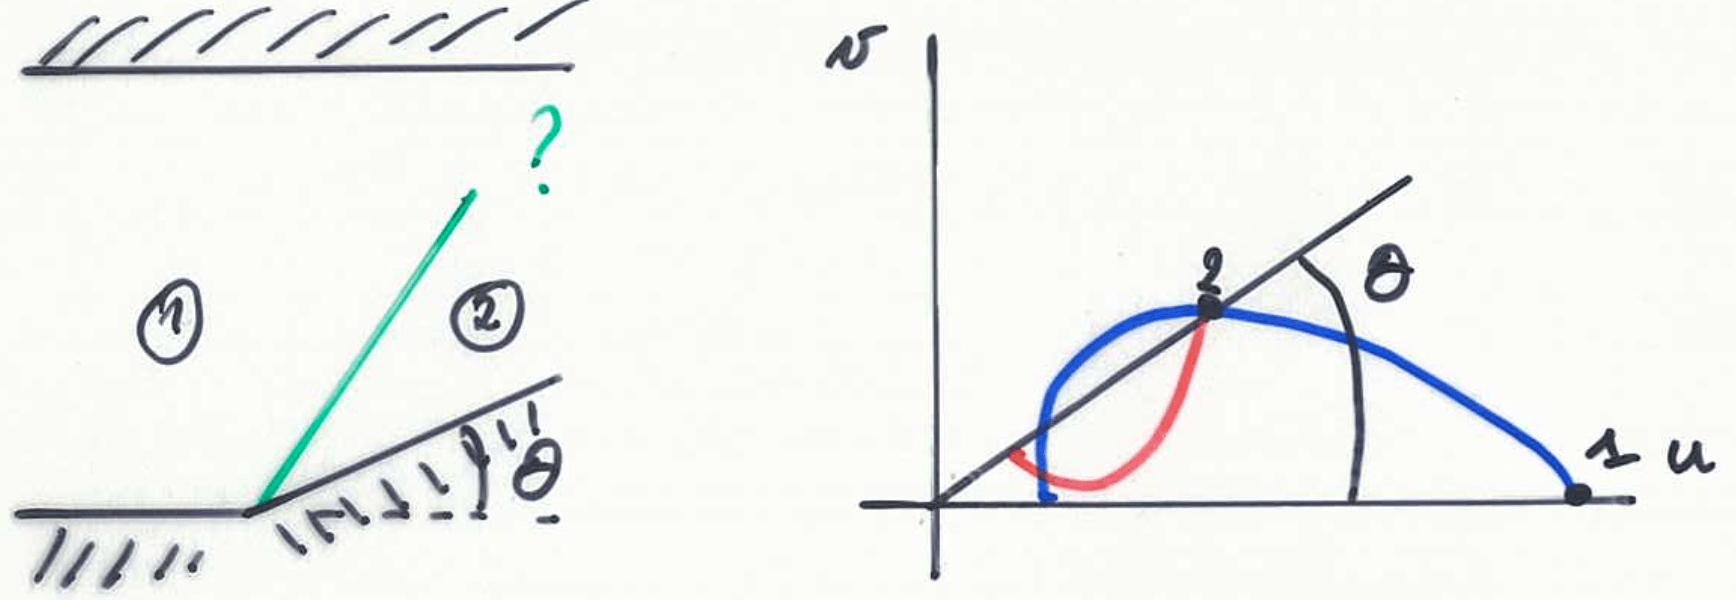
\includegraphics[scale=0.1]{ch9/13}
\captionof{figure}{}
\end{center}

Sometimes, it is not possible to make the reflection with a straight oblique shock. For example if $\theta$ is very high so that the polar curve in 2 has no intersection with the u-axis. In this case, a normal shock appear on the upper wall and has to be connected to the first shock by a bowl shock wave. Another shock appears since the velocity in 3 and 2' must have the same direction (see crossing) and can be not straight. The same can occur for shocks crossing as shown below.

\begin{center}
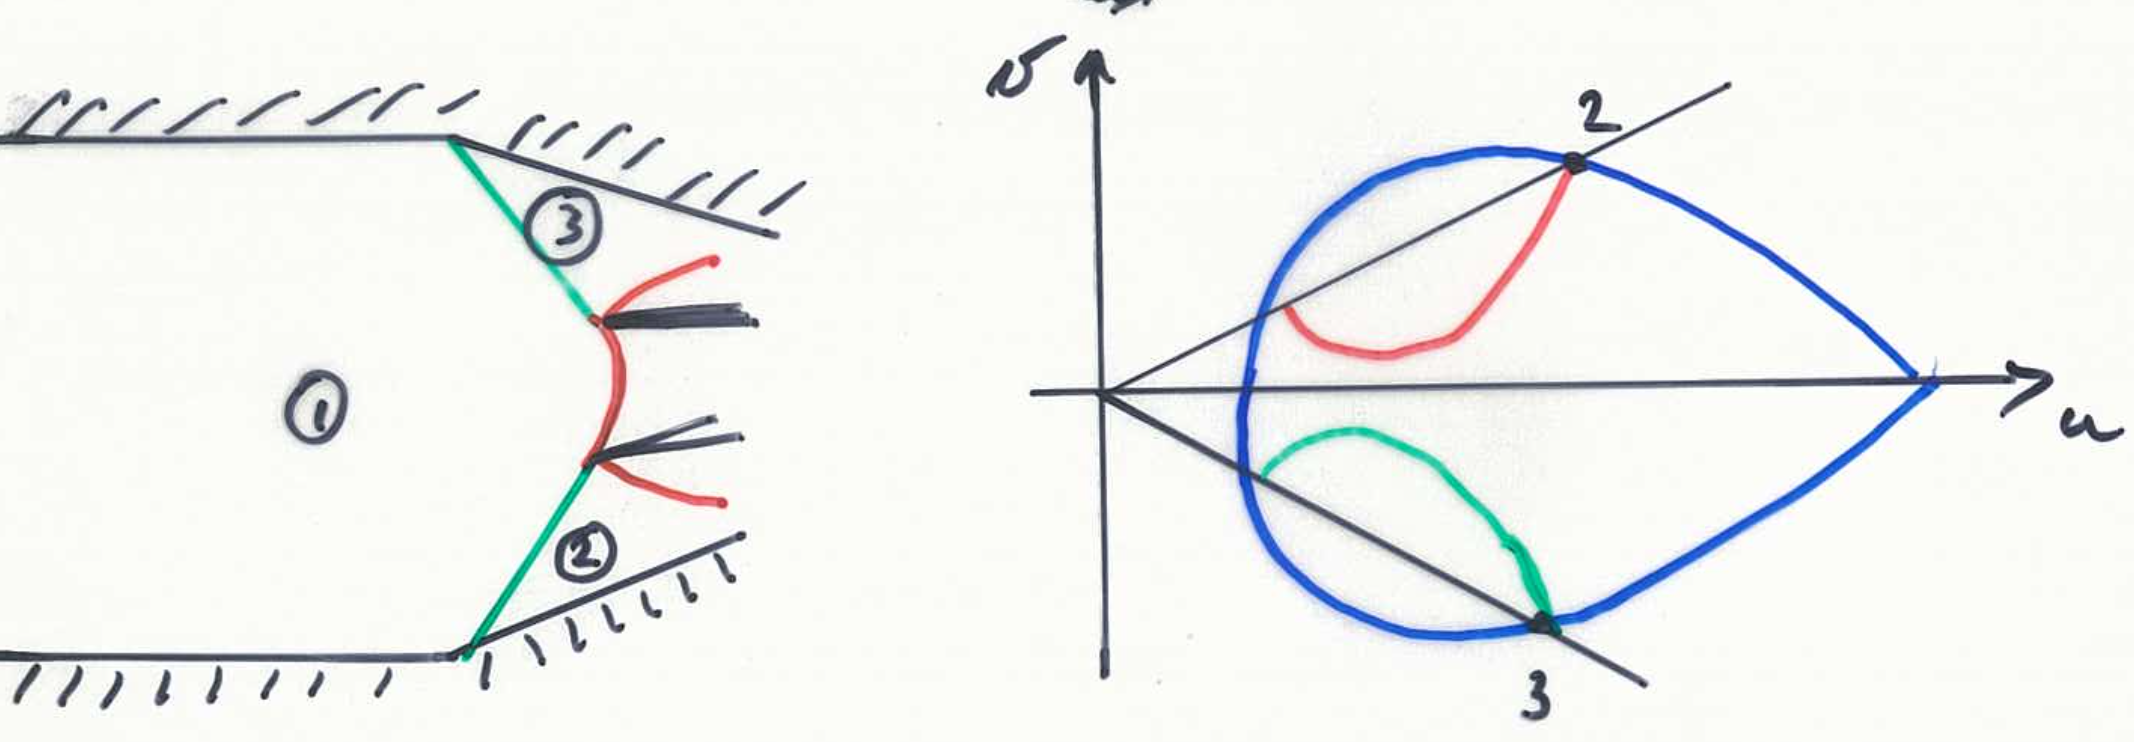
\includegraphics[scale=0.1]{ch9/14}
\captionof{figure}{}
\end{center} 

\section{Crossing of shocks of the same family}
	\begin{center}
\begin{minipage}{0.33\textwidth}
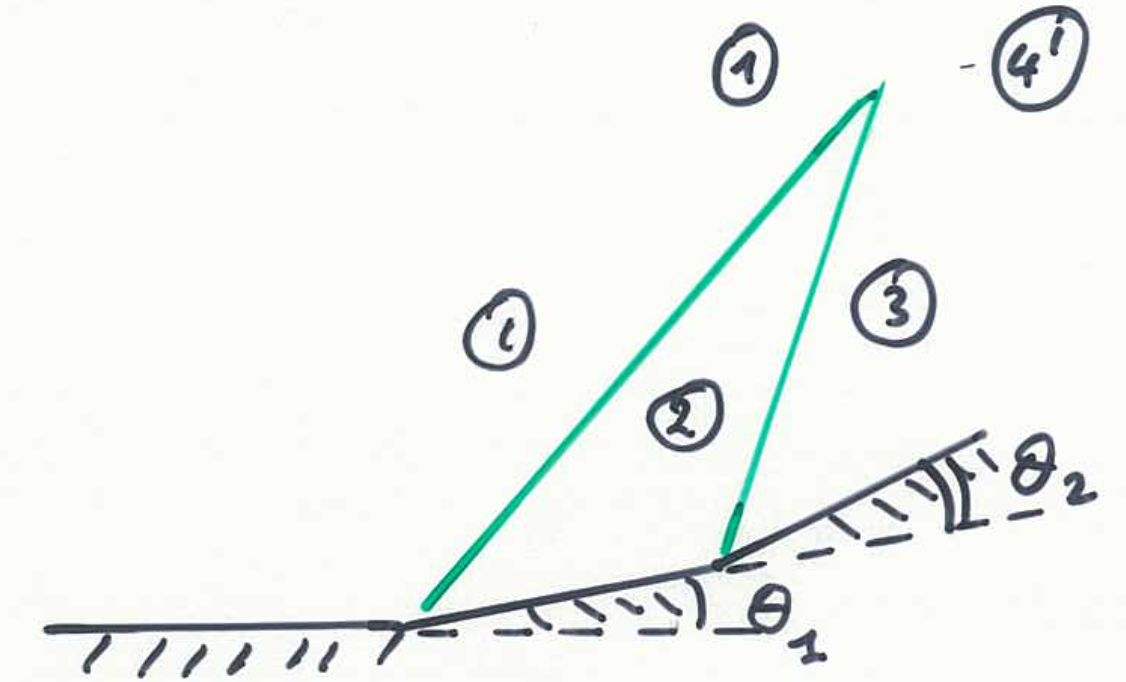
\includegraphics[scale=0.1]{ch9/15}
\captionof{figure}{}
\end{minipage}
\begin{minipage}{0.4\textwidth}
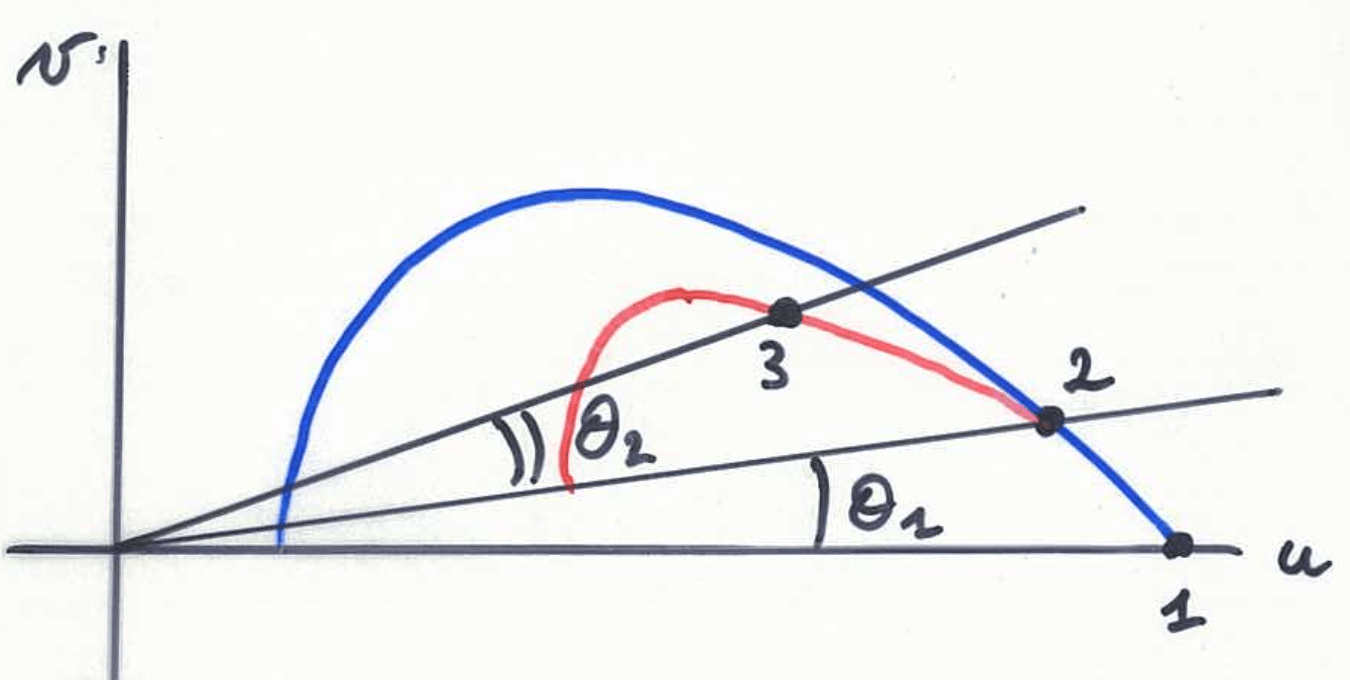
\includegraphics[scale=0.1]{ch9/16}
\captionof{figure}{}
\end{minipage}
\begin{minipage}{0.25\textwidth}
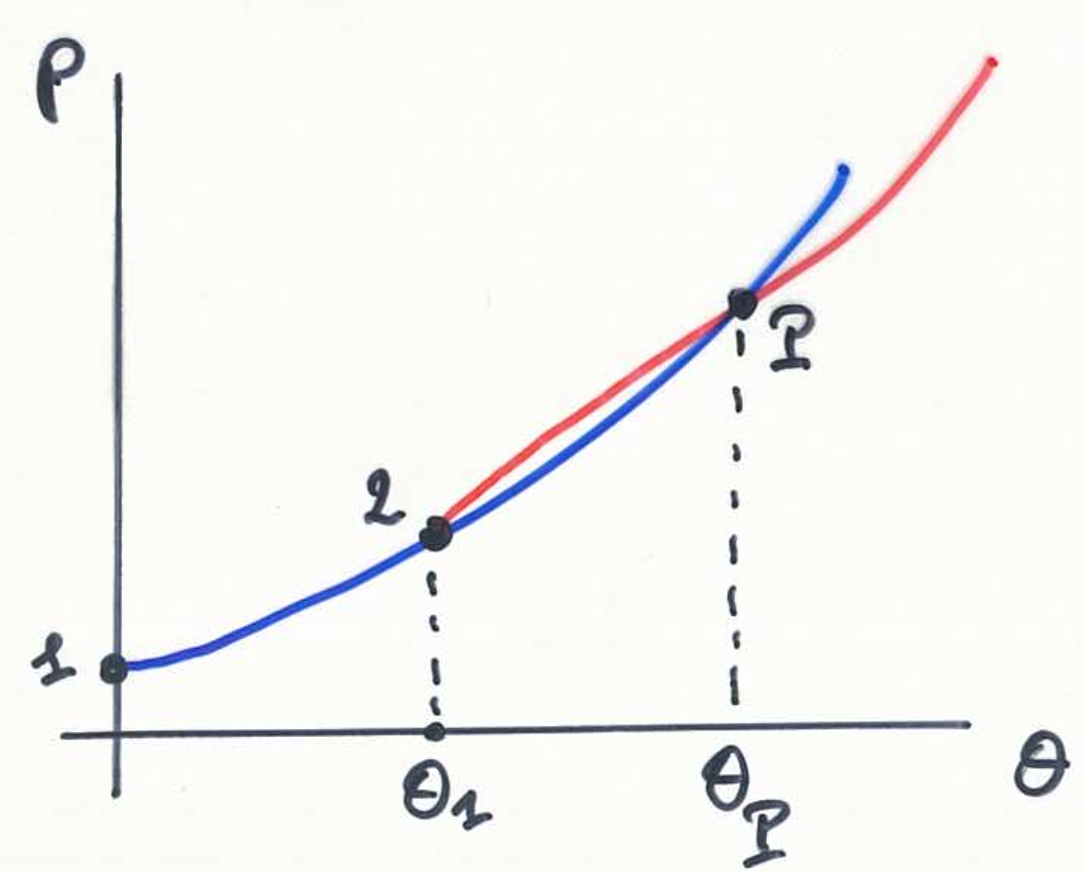
\includegraphics[scale=0.1]{ch9/17}
\captionof{figure}{}
\end{minipage}
\end{center}

Consider the situation represented on the figure. We can draw the u,v curves for situation 1, find situation 2 then plot curve for situation 2 to find 3. As previously, the flows in situation 3 and 1 can meet only if the pressure and the velocity direction are the same. We have thus to look at the $p,\theta$ diagram. There the same reasoning is applied, we use curve of situation 1 to find situation 2, then we use curve of situation 2 to find situation 3. Two cases have to be considered.

\subsubsection{$\bm{\theta _1 + \theta _2 > \theta _P}$}
\begin{center}
\begin{minipage}{0.33\textwidth}
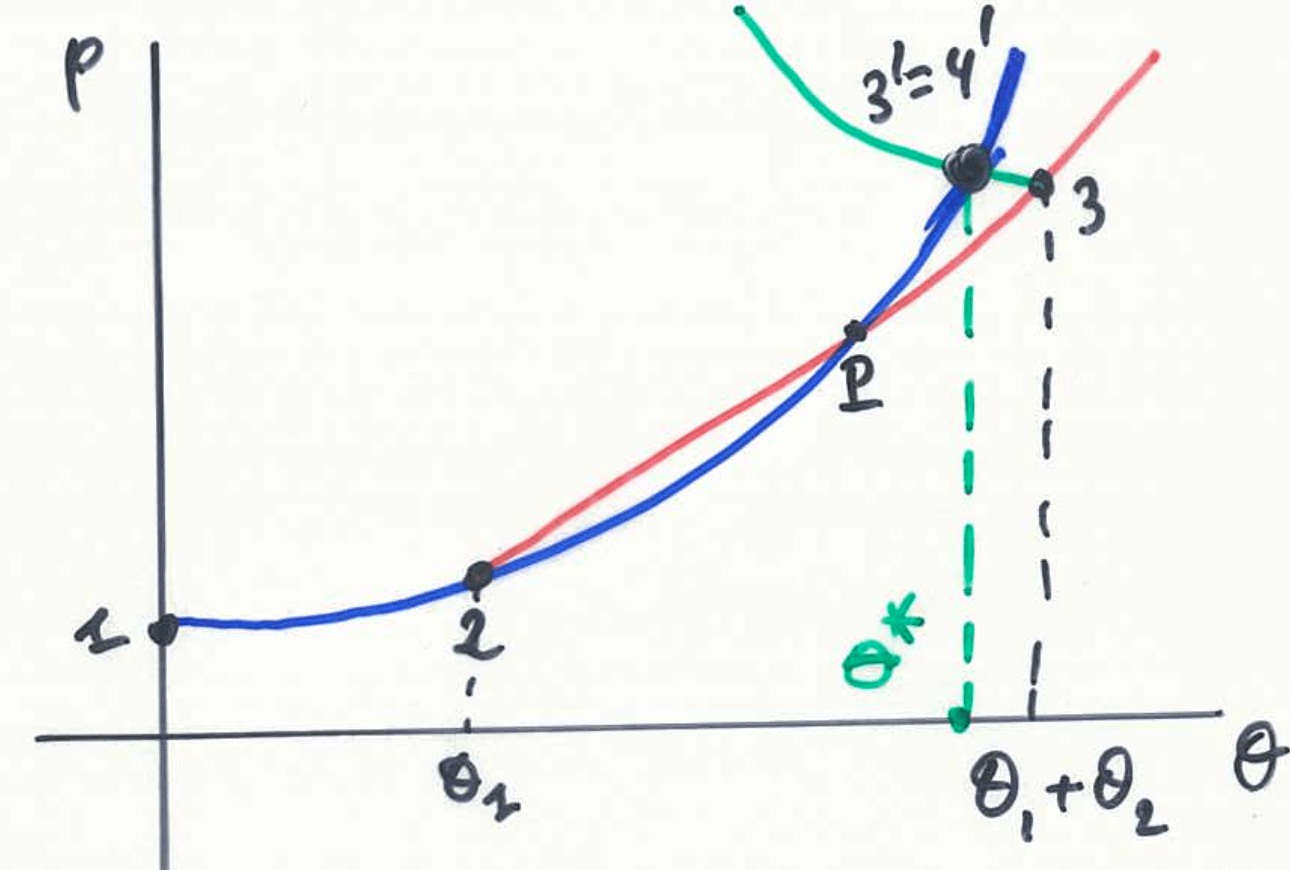
\includegraphics[scale=0.1]{ch9/18}
\captionof{figure}{}
\end{minipage}
\begin{minipage}{0.4\textwidth}
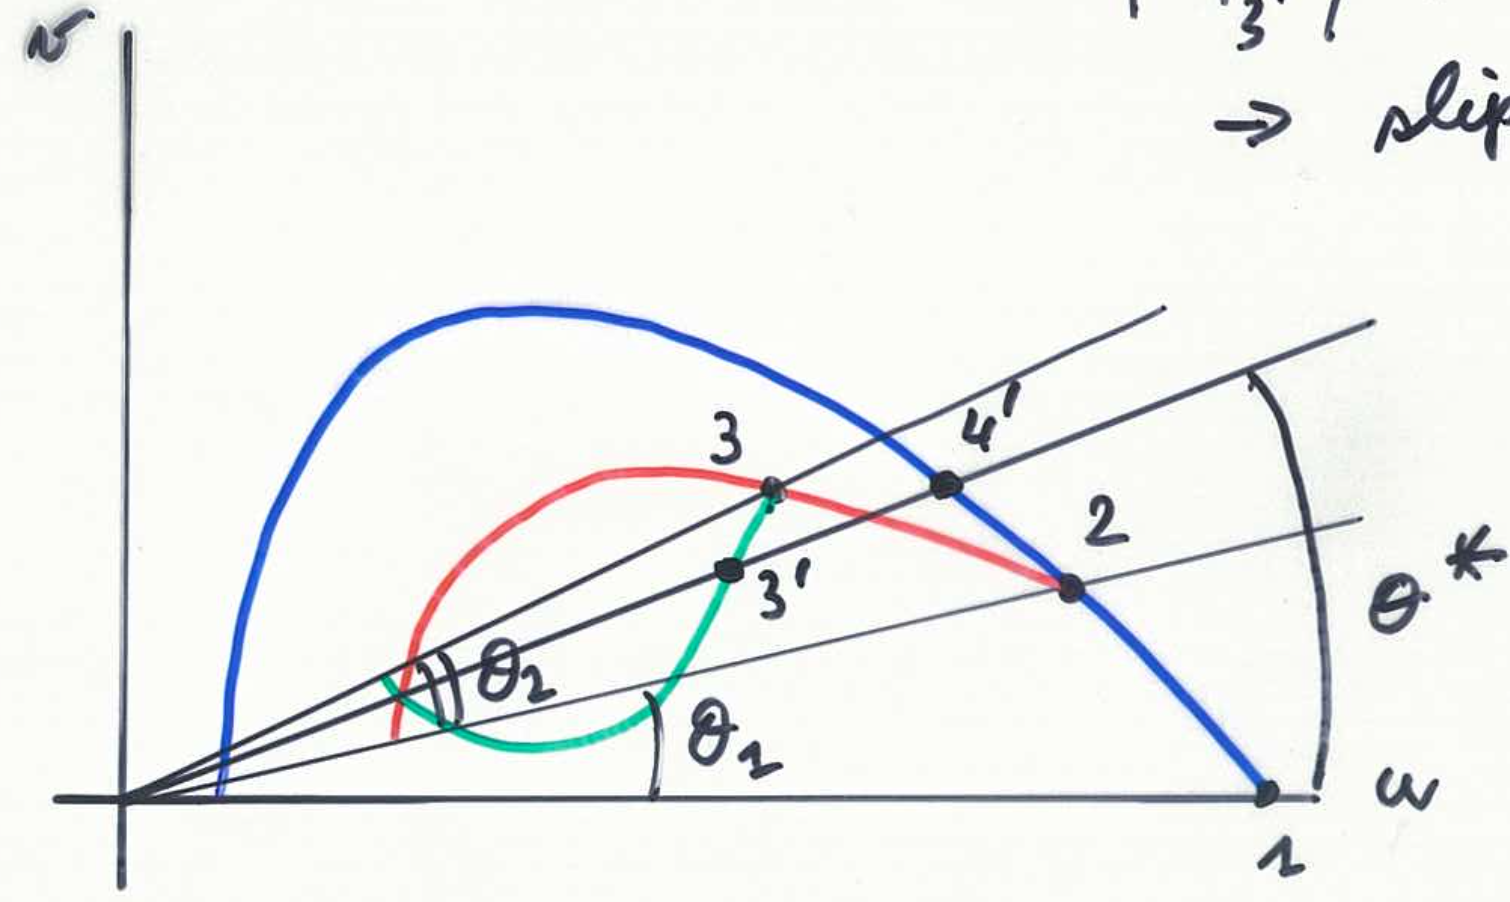
\includegraphics[scale=0.1]{ch9/19}
\captionof{figure}{}
\end{minipage}
\end{center}

Let's denote a particular point by P, intersection of the two chocks. If we are at the right of this point, we could intersect the curve 1 by drawing a curve for situation 3 (reflected shock). This corresponds to the same case as before, where we have a slipping line as the two velocities are different. We find the common angle and we find the velocities on $u,v$ diagram. 

\subsubsection{$\bm{\theta _1 + \theta _2 < \theta _P}$}
\begin{center}
\begin{minipage}{0.33\textwidth}
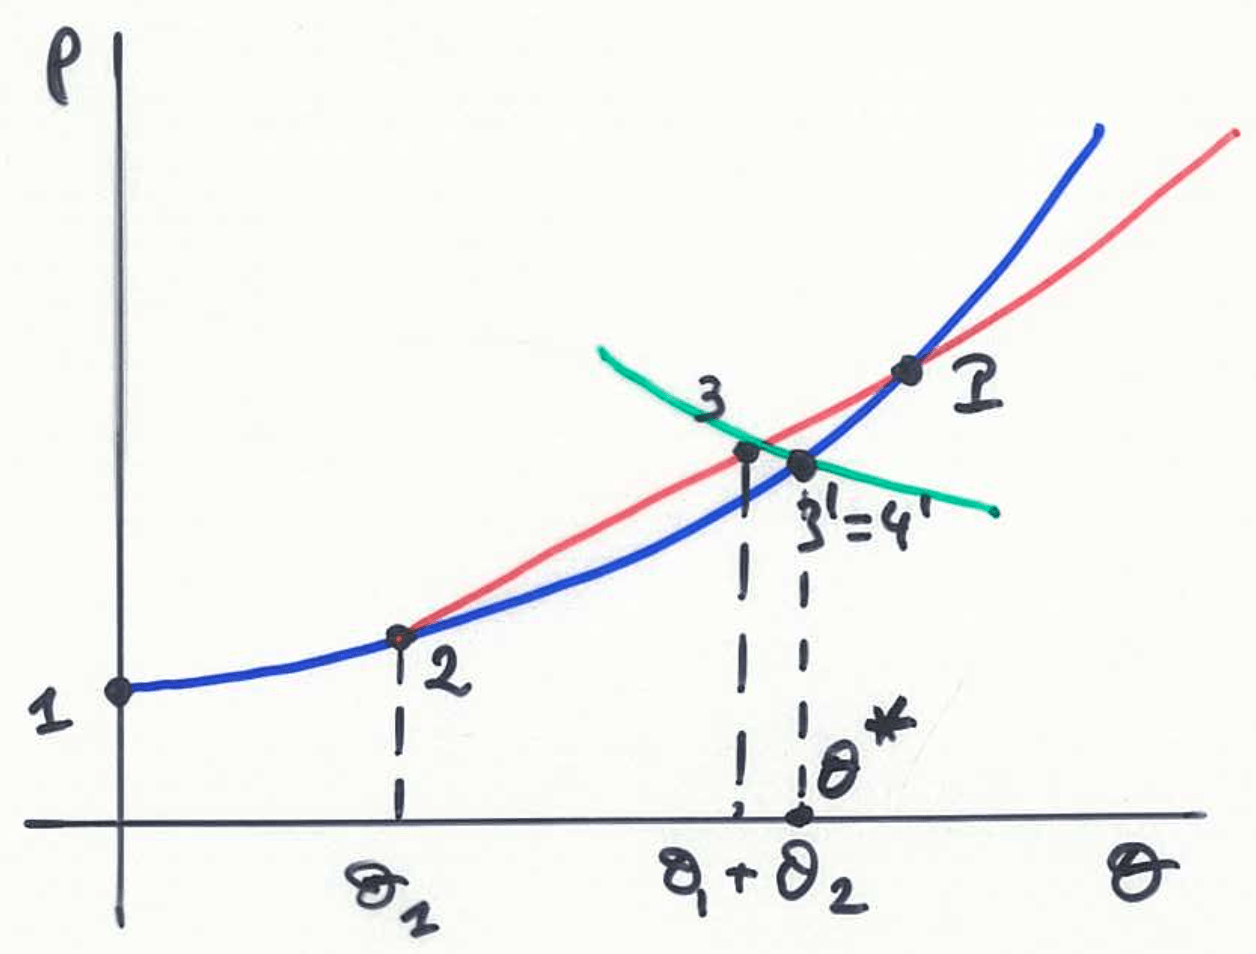
\includegraphics[scale=0.1]{ch9/20}
\captionof{figure}{}
\end{minipage}
\begin{minipage}{0.4\textwidth}
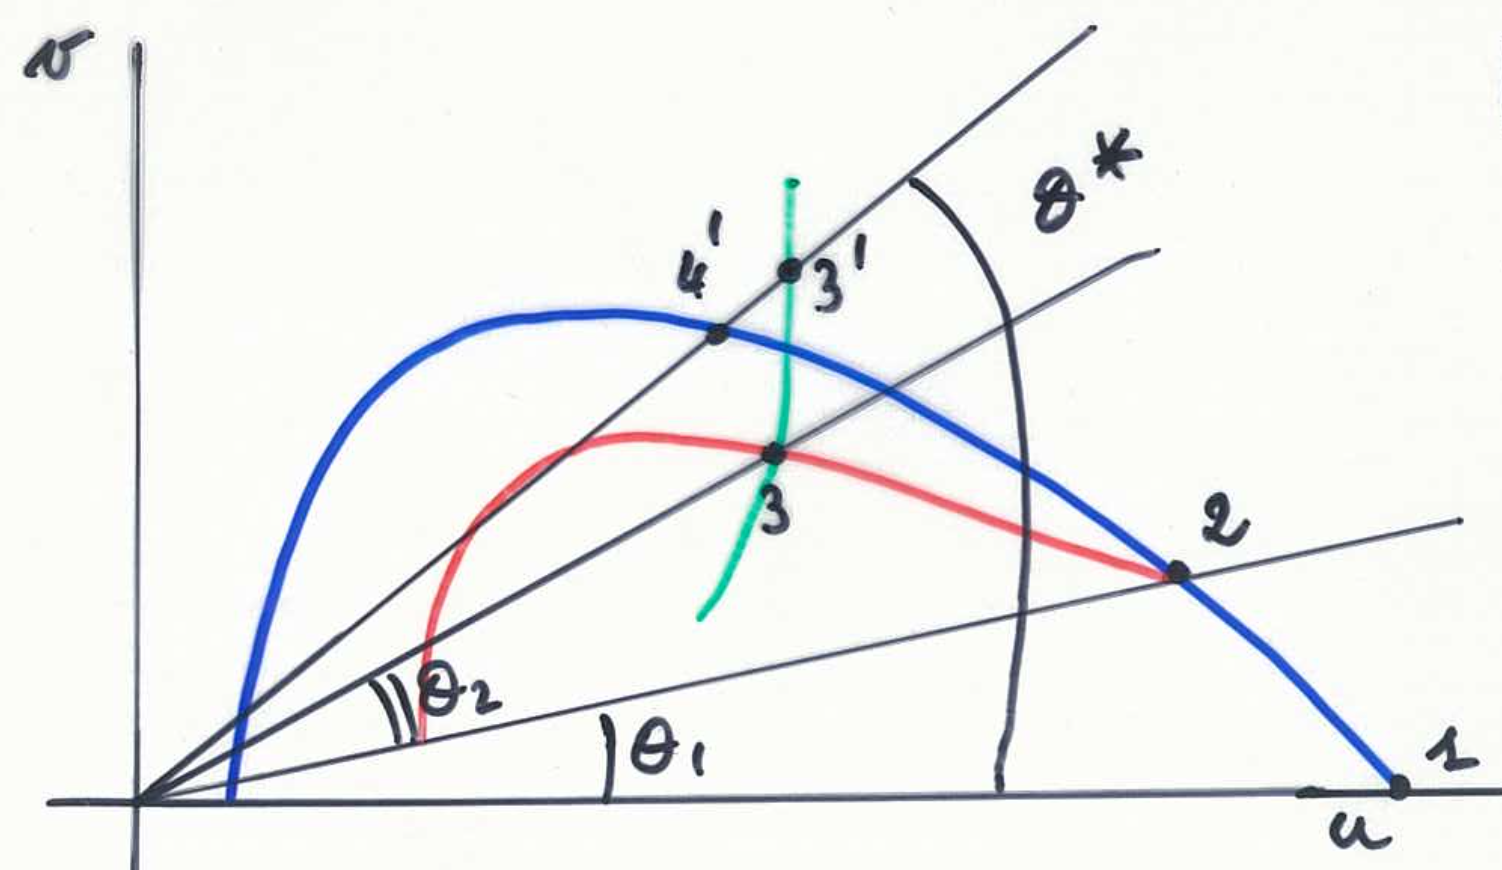
\includegraphics[scale=0.1]{ch9/21}
\captionof{figure}{}
\end{minipage}
\end{center}

If now the situation 3 is in the left of P, the reflected shock cannot allow us to reach the curve 1 since we need to decrease the pressure. The solution for this is to use the traditional Mach waves that are represented like that on the p,$\theta$ diagram. Now we have an intersection, an angle $\theta ^*$ and we can find the velocities. There is also a slipping line. 

\begin{center}
\begin{minipage}{0.33\textwidth}
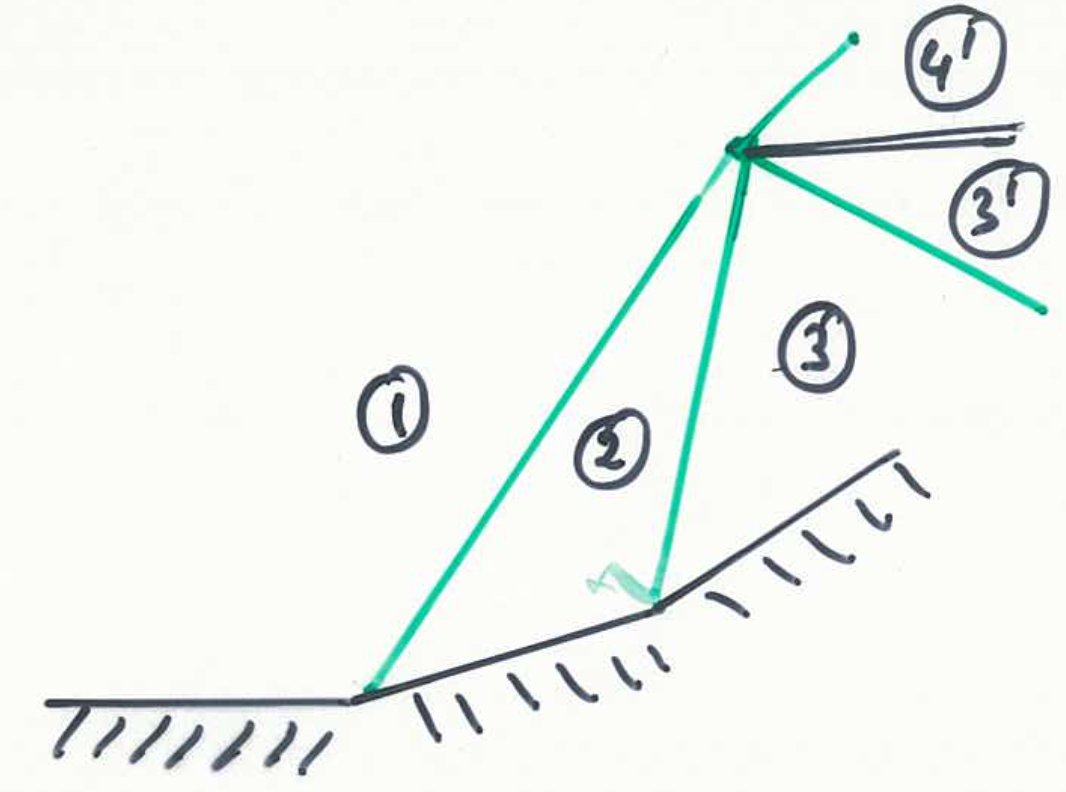
\includegraphics[scale=0.1]{ch9/22}
\captionof{figure}{}
\end{minipage}
\begin{minipage}{0.4\textwidth}
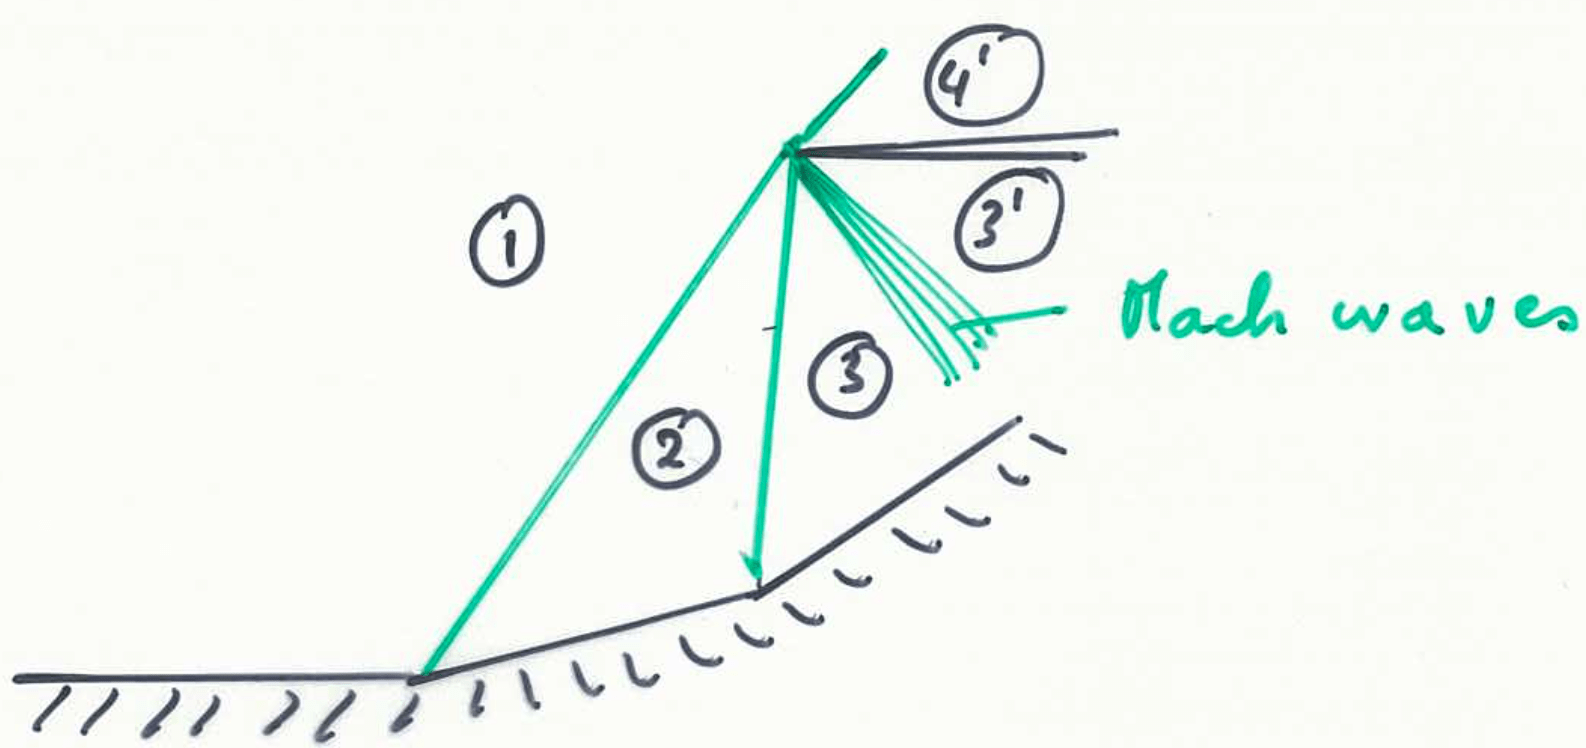
\includegraphics[scale=0.1]{ch9/23}
\captionof{figure}{}
\end{minipage}
\end{center}

\begin{center}
\theor{
\textbf{This was the end of this beautiful course, I hope you enjoyed every page of this summary and please correct/update it to help future generations. Good luck.}
}
\end{center}